
% Inherit from the specified cell style.

% Default to the notebook output style

    


% Inherit from the specified cell style.




    
\documentclass[letter]{article}

    
    
% \usepackage{stix}
% \usepackage[scr]{rsfso}
% \usepackage{bm}

\usepackage[T1]{fontenc}
% Nicer default font than Computer Modern for most use cases
\usepackage{palatino}
\usepackage{eulervm}
\usepackage[bb=boondox]{mathalfa}

% Basic figure setup, for now with no caption control since it's done
% automatically by Pandoc (which extracts ![](path) syntax from Markdown).
\usepackage{graphicx}
% We will generate all images so they have a width \maxwidth. This means
% that they will get their normal width if they fit onto the page, but
% are scaled down if they would overflow the margins.
\makeatletter
\def\maxwidth{\ifdim\Gin@nat@width>\linewidth\linewidth
\else\Gin@nat@width\fi}
\makeatother
\let\Oldincludegraphics\includegraphics
% Set max figure width to be 80% of text width, for now hardcoded.
\renewcommand{\includegraphics}[1]{\Oldincludegraphics[width=0.98\maxwidth]{#1}}
% Ensure that by default, figures have no caption (until we provide a
% proper Figure object with a Caption API and a way to capture that
% in the conversion process - todo).
\usepackage{caption}
% \DeclareCaptionLabelFormat{nolabel}{}
\captionsetup{width=0.95\textwidth,labelfont=bf,textfont=it}

\usepackage{adjustbox} % Used to constrain images to a maximum size 
\usepackage{xcolor} % Allow colors to be defined
\usepackage{enumerate} % Needed for markdown enumerations to work
\usepackage{geometry} % Used to adjust the document margins
\usepackage{amsmath} % Equations
\usepackage{amssymb} % Equations
\usepackage{textcomp} % defines textquotesingle
% Hack from http://tex.stackexchange.com/a/47451/13684:
\AtBeginDocument{%
    \def\PYZsq{\textquotesingle}% Upright quotes in Pygmentized code
}
\usepackage{upquote} % Upright quotes for verbatim code
\usepackage{eurosym} % defines \euro
\usepackage[mathletters]{ucs} % Extended unicode (utf-8) support
\usepackage[utf8x]{inputenc} % Allow utf-8 characters in the tex document
\usepackage{fancyvrb} % verbatim replacement that allows latex
\usepackage{grffile} % extends the file name processing of package graphics 
                     % to support a larger range 
% The hyperref package gives us a pdf with properly built
% internal navigation ('pdf bookmarks' for the table of contents,
% internal cross-reference links, web links for URLs, etc.)
\usepackage{hyperref}
\usepackage{longtable} % longtable support required by pandoc >1.10
\usepackage{booktabs}  % table support for pandoc > 1.12.2
\usepackage[normalem]{ulem} % ulem is needed to support strikethroughs (\sout)
                            % normalem makes italics be italics, not underlines
\usepackage{newunicodechar}
\usepackage{natbib}
\usepackage{cancel}
\usepackage{authblk}

\usepackage[doublespacing]{setspace}


    
    
    
    % Colors for the hyperref package
    \definecolor{urlcolor}{rgb}{0,.145,.698}
    \definecolor{linkcolor}{rgb}{.71,0.21,0.01}
    \definecolor{citecolor}{rgb}{.12,.54,.11}

    % ANSI colors
    \definecolor{ansi-black}{HTML}{3E424D}
    \definecolor{ansi-black-intense}{HTML}{282C36}
    \definecolor{ansi-red}{HTML}{E75C58}
    \definecolor{ansi-red-intense}{HTML}{B22B31}
    \definecolor{ansi-green}{HTML}{00A250}
    \definecolor{ansi-green-intense}{HTML}{007427}
    \definecolor{ansi-yellow}{HTML}{DDB62B}
    \definecolor{ansi-yellow-intense}{HTML}{B27D12}
    \definecolor{ansi-blue}{HTML}{208FFB}
    \definecolor{ansi-blue-intense}{HTML}{0065CA}
    \definecolor{ansi-magenta}{HTML}{D160C4}
    \definecolor{ansi-magenta-intense}{HTML}{A03196}
    \definecolor{ansi-cyan}{HTML}{60C6C8}
    \definecolor{ansi-cyan-intense}{HTML}{258F8F}
    \definecolor{ansi-white}{HTML}{C5C1B4}
    \definecolor{ansi-white-intense}{HTML}{A1A6B2}

    % commands and environments needed by pandoc snippets
    % extracted from the output of `pandoc -s`
    \providecommand{\tightlist}{%
      \setlength{\itemsep}{0pt}\setlength{\parskip}{0pt}}
    \DefineVerbatimEnvironment{Highlighting}{Verbatim}{commandchars=\\\{\}}
    % Add ',fontsize=\small' for more characters per line
    \newenvironment{Shaded}{}{}
    \newcommand{\KeywordTok}[1]{\textcolor[rgb]{0.00,0.44,0.13}{\textbf{{#1}}}}
    \newcommand{\DataTypeTok}[1]{\textcolor[rgb]{0.56,0.13,0.00}{{#1}}}
    \newcommand{\DecValTok}[1]{\textcolor[rgb]{0.25,0.63,0.44}{{#1}}}
    \newcommand{\BaseNTok}[1]{\textcolor[rgb]{0.25,0.63,0.44}{{#1}}}
    \newcommand{\FloatTok}[1]{\textcolor[rgb]{0.25,0.63,0.44}{{#1}}}
    \newcommand{\CharTok}[1]{\textcolor[rgb]{0.25,0.44,0.63}{{#1}}}
    \newcommand{\StringTok}[1]{\textcolor[rgb]{0.25,0.44,0.63}{{#1}}}
    \newcommand{\CommentTok}[1]{\textcolor[rgb]{0.38,0.63,0.69}{\textit{{#1}}}}
    \newcommand{\OtherTok}[1]{\textcolor[rgb]{0.00,0.44,0.13}{{#1}}}
    \newcommand{\AlertTok}[1]{\textcolor[rgb]{1.00,0.00,0.00}{\textbf{{#1}}}}
    \newcommand{\FunctionTok}[1]{\textcolor[rgb]{0.02,0.16,0.49}{{#1}}}
    \newcommand{\RegionMarkerTok}[1]{{#1}}
    \newcommand{\ErrorTok}[1]{\textcolor[rgb]{1.00,0.00,0.00}{\textbf{{#1}}}}
    \newcommand{\NormalTok}[1]{{#1}}
    
    % Additional commands for more recent versions of Pandoc
    \newcommand{\ConstantTok}[1]{\textcolor[rgb]{0.53,0.00,0.00}{{#1}}}
    \newcommand{\SpecialCharTok}[1]{\textcolor[rgb]{0.25,0.44,0.63}{{#1}}}
    \newcommand{\VerbatimStringTok}[1]{\textcolor[rgb]{0.25,0.44,0.63}{{#1}}}
    \newcommand{\SpecialStringTok}[1]{\textcolor[rgb]{0.73,0.40,0.53}{{#1}}}
    \newcommand{\ImportTok}[1]{{#1}}
    \newcommand{\DocumentationTok}[1]{\textcolor[rgb]{0.73,0.13,0.13}{\textit{{#1}}}}
    \newcommand{\AnnotationTok}[1]{\textcolor[rgb]{0.38,0.63,0.69}{\textbf{\textit{{#1}}}}}
    \newcommand{\CommentVarTok}[1]{\textcolor[rgb]{0.38,0.63,0.69}{\textbf{\textit{{#1}}}}}
    \newcommand{\VariableTok}[1]{\textcolor[rgb]{0.10,0.09,0.49}{{#1}}}
    \newcommand{\ControlFlowTok}[1]{\textcolor[rgb]{0.00,0.44,0.13}{\textbf{{#1}}}}
    \newcommand{\OperatorTok}[1]{\textcolor[rgb]{0.40,0.40,0.40}{{#1}}}
    \newcommand{\BuiltInTok}[1]{{#1}}
    \newcommand{\ExtensionTok}[1]{{#1}}
    \newcommand{\PreprocessorTok}[1]{\textcolor[rgb]{0.74,0.48,0.00}{{#1}}}
    \newcommand{\AttributeTok}[1]{\textcolor[rgb]{0.49,0.56,0.16}{{#1}}}
    \newcommand{\InformationTok}[1]{\textcolor[rgb]{0.38,0.63,0.69}{\textbf{\textit{{#1}}}}}
    \newcommand{\WarningTok}[1]{\textcolor[rgb]{0.38,0.63,0.69}{\textbf{\textit{{#1}}}}}
    
    
    % Define a nice break command that doesn't care if a line doesn't already
    % exist.
    \def\br{\hspace*{\fill} \\* }
    % Math Jax compatability definitions
    \def\gt{>}
    \def\lt{<}
    % Document parameters
    
	\title{
		Bias correction in daily maximum and minimum temperature measurements through Gaussian process modeling
		}

    
    
\author[*]{Maxime Rischard}
\affil[*]{Department of Statistics, Harvard University}
% \affil[**]{National Center for Atmospheric Research}

    

    % Pygments definitions
    
\makeatletter
\def\PY@reset{\let\PY@it=\relax \let\PY@bf=\relax%
    \let\PY@ul=\relax \let\PY@tc=\relax%
    \let\PY@bc=\relax \let\PY@ff=\relax}
\def\PY@tok#1{\csname PY@tok@#1\endcsname}
\def\PY@toks#1+{\ifx\relax#1\empty\else%
    \PY@tok{#1}\expandafter\PY@toks\fi}
\def\PY@do#1{\PY@bc{\PY@tc{\PY@ul{%
    \PY@it{\PY@bf{\PY@ff{#1}}}}}}}
\def\PY#1#2{\PY@reset\PY@toks#1+\relax+\PY@do{#2}}

\expandafter\def\csname PY@tok@ss\endcsname{\def\PY@tc##1{\textcolor[rgb]{0.10,0.09,0.49}{##1}}}
\expandafter\def\csname PY@tok@c1\endcsname{\let\PY@it=\textit\def\PY@tc##1{\textcolor[rgb]{0.25,0.50,0.50}{##1}}}
\expandafter\def\csname PY@tok@cpf\endcsname{\let\PY@it=\textit\def\PY@tc##1{\textcolor[rgb]{0.25,0.50,0.50}{##1}}}
\expandafter\def\csname PY@tok@sd\endcsname{\let\PY@it=\textit\def\PY@tc##1{\textcolor[rgb]{0.73,0.13,0.13}{##1}}}
\expandafter\def\csname PY@tok@gs\endcsname{\let\PY@bf=\textbf}
\expandafter\def\csname PY@tok@m\endcsname{\def\PY@tc##1{\textcolor[rgb]{0.40,0.40,0.40}{##1}}}
\expandafter\def\csname PY@tok@kr\endcsname{\let\PY@bf=\textbf\def\PY@tc##1{\textcolor[rgb]{0.00,0.50,0.00}{##1}}}
\expandafter\def\csname PY@tok@o\endcsname{\def\PY@tc##1{\textcolor[rgb]{0.40,0.40,0.40}{##1}}}
\expandafter\def\csname PY@tok@gr\endcsname{\def\PY@tc##1{\textcolor[rgb]{1.00,0.00,0.00}{##1}}}
\expandafter\def\csname PY@tok@cp\endcsname{\def\PY@tc##1{\textcolor[rgb]{0.74,0.48,0.00}{##1}}}
\expandafter\def\csname PY@tok@na\endcsname{\def\PY@tc##1{\textcolor[rgb]{0.49,0.56,0.16}{##1}}}
\expandafter\def\csname PY@tok@sh\endcsname{\def\PY@tc##1{\textcolor[rgb]{0.73,0.13,0.13}{##1}}}
\expandafter\def\csname PY@tok@nt\endcsname{\let\PY@bf=\textbf\def\PY@tc##1{\textcolor[rgb]{0.00,0.50,0.00}{##1}}}
\expandafter\def\csname PY@tok@k\endcsname{\let\PY@bf=\textbf\def\PY@tc##1{\textcolor[rgb]{0.00,0.50,0.00}{##1}}}
\expandafter\def\csname PY@tok@w\endcsname{\def\PY@tc##1{\textcolor[rgb]{0.73,0.73,0.73}{##1}}}
\expandafter\def\csname PY@tok@mi\endcsname{\def\PY@tc##1{\textcolor[rgb]{0.40,0.40,0.40}{##1}}}
\expandafter\def\csname PY@tok@mf\endcsname{\def\PY@tc##1{\textcolor[rgb]{0.40,0.40,0.40}{##1}}}
\expandafter\def\csname PY@tok@kp\endcsname{\def\PY@tc##1{\textcolor[rgb]{0.00,0.50,0.00}{##1}}}
\expandafter\def\csname PY@tok@ni\endcsname{\let\PY@bf=\textbf\def\PY@tc##1{\textcolor[rgb]{0.60,0.60,0.60}{##1}}}
\expandafter\def\csname PY@tok@cm\endcsname{\let\PY@it=\textit\def\PY@tc##1{\textcolor[rgb]{0.25,0.50,0.50}{##1}}}
\expandafter\def\csname PY@tok@gd\endcsname{\def\PY@tc##1{\textcolor[rgb]{0.63,0.00,0.00}{##1}}}
\expandafter\def\csname PY@tok@ge\endcsname{\let\PY@it=\textit}
\expandafter\def\csname PY@tok@vm\endcsname{\def\PY@tc##1{\textcolor[rgb]{0.10,0.09,0.49}{##1}}}
\expandafter\def\csname PY@tok@bp\endcsname{\def\PY@tc##1{\textcolor[rgb]{0.00,0.50,0.00}{##1}}}
\expandafter\def\csname PY@tok@gh\endcsname{\let\PY@bf=\textbf\def\PY@tc##1{\textcolor[rgb]{0.00,0.00,0.50}{##1}}}
\expandafter\def\csname PY@tok@nf\endcsname{\def\PY@tc##1{\textcolor[rgb]{0.00,0.00,1.00}{##1}}}
\expandafter\def\csname PY@tok@nl\endcsname{\def\PY@tc##1{\textcolor[rgb]{0.63,0.63,0.00}{##1}}}
\expandafter\def\csname PY@tok@vi\endcsname{\def\PY@tc##1{\textcolor[rgb]{0.10,0.09,0.49}{##1}}}
\expandafter\def\csname PY@tok@sa\endcsname{\def\PY@tc##1{\textcolor[rgb]{0.73,0.13,0.13}{##1}}}
\expandafter\def\csname PY@tok@sb\endcsname{\def\PY@tc##1{\textcolor[rgb]{0.73,0.13,0.13}{##1}}}
\expandafter\def\csname PY@tok@sx\endcsname{\def\PY@tc##1{\textcolor[rgb]{0.00,0.50,0.00}{##1}}}
\expandafter\def\csname PY@tok@gu\endcsname{\let\PY@bf=\textbf\def\PY@tc##1{\textcolor[rgb]{0.50,0.00,0.50}{##1}}}
\expandafter\def\csname PY@tok@vc\endcsname{\def\PY@tc##1{\textcolor[rgb]{0.10,0.09,0.49}{##1}}}
\expandafter\def\csname PY@tok@ch\endcsname{\let\PY@it=\textit\def\PY@tc##1{\textcolor[rgb]{0.25,0.50,0.50}{##1}}}
\expandafter\def\csname PY@tok@ow\endcsname{\let\PY@bf=\textbf\def\PY@tc##1{\textcolor[rgb]{0.67,0.13,1.00}{##1}}}
\expandafter\def\csname PY@tok@gt\endcsname{\def\PY@tc##1{\textcolor[rgb]{0.00,0.27,0.87}{##1}}}
\expandafter\def\csname PY@tok@s1\endcsname{\def\PY@tc##1{\textcolor[rgb]{0.73,0.13,0.13}{##1}}}
\expandafter\def\csname PY@tok@gp\endcsname{\let\PY@bf=\textbf\def\PY@tc##1{\textcolor[rgb]{0.00,0.00,0.50}{##1}}}
\expandafter\def\csname PY@tok@mo\endcsname{\def\PY@tc##1{\textcolor[rgb]{0.40,0.40,0.40}{##1}}}
\expandafter\def\csname PY@tok@gi\endcsname{\def\PY@tc##1{\textcolor[rgb]{0.00,0.63,0.00}{##1}}}
\expandafter\def\csname PY@tok@se\endcsname{\let\PY@bf=\textbf\def\PY@tc##1{\textcolor[rgb]{0.73,0.40,0.13}{##1}}}
\expandafter\def\csname PY@tok@il\endcsname{\def\PY@tc##1{\textcolor[rgb]{0.40,0.40,0.40}{##1}}}
\expandafter\def\csname PY@tok@go\endcsname{\def\PY@tc##1{\textcolor[rgb]{0.53,0.53,0.53}{##1}}}
\expandafter\def\csname PY@tok@vg\endcsname{\def\PY@tc##1{\textcolor[rgb]{0.10,0.09,0.49}{##1}}}
\expandafter\def\csname PY@tok@s\endcsname{\def\PY@tc##1{\textcolor[rgb]{0.73,0.13,0.13}{##1}}}
\expandafter\def\csname PY@tok@nd\endcsname{\def\PY@tc##1{\textcolor[rgb]{0.67,0.13,1.00}{##1}}}
\expandafter\def\csname PY@tok@c\endcsname{\let\PY@it=\textit\def\PY@tc##1{\textcolor[rgb]{0.25,0.50,0.50}{##1}}}
\expandafter\def\csname PY@tok@si\endcsname{\let\PY@bf=\textbf\def\PY@tc##1{\textcolor[rgb]{0.73,0.40,0.53}{##1}}}
\expandafter\def\csname PY@tok@sc\endcsname{\def\PY@tc##1{\textcolor[rgb]{0.73,0.13,0.13}{##1}}}
\expandafter\def\csname PY@tok@fm\endcsname{\def\PY@tc##1{\textcolor[rgb]{0.00,0.00,1.00}{##1}}}
\expandafter\def\csname PY@tok@nn\endcsname{\let\PY@bf=\textbf\def\PY@tc##1{\textcolor[rgb]{0.00,0.00,1.00}{##1}}}
\expandafter\def\csname PY@tok@ne\endcsname{\let\PY@bf=\textbf\def\PY@tc##1{\textcolor[rgb]{0.82,0.25,0.23}{##1}}}
\expandafter\def\csname PY@tok@sr\endcsname{\def\PY@tc##1{\textcolor[rgb]{0.73,0.40,0.53}{##1}}}
\expandafter\def\csname PY@tok@mh\endcsname{\def\PY@tc##1{\textcolor[rgb]{0.40,0.40,0.40}{##1}}}
\expandafter\def\csname PY@tok@no\endcsname{\def\PY@tc##1{\textcolor[rgb]{0.53,0.00,0.00}{##1}}}
\expandafter\def\csname PY@tok@mb\endcsname{\def\PY@tc##1{\textcolor[rgb]{0.40,0.40,0.40}{##1}}}
\expandafter\def\csname PY@tok@kn\endcsname{\let\PY@bf=\textbf\def\PY@tc##1{\textcolor[rgb]{0.00,0.50,0.00}{##1}}}
\expandafter\def\csname PY@tok@kd\endcsname{\let\PY@bf=\textbf\def\PY@tc##1{\textcolor[rgb]{0.00,0.50,0.00}{##1}}}
\expandafter\def\csname PY@tok@s2\endcsname{\def\PY@tc##1{\textcolor[rgb]{0.73,0.13,0.13}{##1}}}
\expandafter\def\csname PY@tok@nb\endcsname{\def\PY@tc##1{\textcolor[rgb]{0.00,0.50,0.00}{##1}}}
\expandafter\def\csname PY@tok@nc\endcsname{\let\PY@bf=\textbf\def\PY@tc##1{\textcolor[rgb]{0.00,0.00,1.00}{##1}}}
\expandafter\def\csname PY@tok@kt\endcsname{\def\PY@tc##1{\textcolor[rgb]{0.69,0.00,0.25}{##1}}}
\expandafter\def\csname PY@tok@kc\endcsname{\let\PY@bf=\textbf\def\PY@tc##1{\textcolor[rgb]{0.00,0.50,0.00}{##1}}}
\expandafter\def\csname PY@tok@nv\endcsname{\def\PY@tc##1{\textcolor[rgb]{0.10,0.09,0.49}{##1}}}
\expandafter\def\csname PY@tok@err\endcsname{\def\PY@bc##1{\setlength{\fboxsep}{0pt}\fcolorbox[rgb]{1.00,0.00,0.00}{1,1,1}{\strut ##1}}}
\expandafter\def\csname PY@tok@dl\endcsname{\def\PY@tc##1{\textcolor[rgb]{0.73,0.13,0.13}{##1}}}
\expandafter\def\csname PY@tok@cs\endcsname{\let\PY@it=\textit\def\PY@tc##1{\textcolor[rgb]{0.25,0.50,0.50}{##1}}}

\def\PYZbs{\char`\\}
\def\PYZus{\char`\_}
\def\PYZob{\char`\{}
\def\PYZcb{\char`\}}
\def\PYZca{\char`\^}
\def\PYZam{\char`\&}
\def\PYZlt{\char`\<}
\def\PYZgt{\char`\>}
\def\PYZsh{\char`\#}
\def\PYZpc{\char`\%}
\def\PYZdl{\char`\$}
\def\PYZhy{\char`\-}
\def\PYZsq{\char`\'}
\def\PYZdq{\char`\"}
\def\PYZti{\char`\~}
% for compatibility with earlier versions
\def\PYZat{@}
\def\PYZlb{[}
\def\PYZrb{]}
\makeatother


    % Exact colors from NB
    \definecolor{incolor}{rgb}{0.0, 0.0, 0.5}
    \definecolor{outcolor}{rgb}{0.545, 0.0, 0.0}


    \newcommand{\genericdel}[3]{%
      \left#1#3\right#2
    }
    \newcommand{\del}[1]{\genericdel(){#1}}
    \newcommand{\sbr}[1]{\genericdel[]{#1}}
    \newcommand{\cbr}[1]{\genericdel\{\}{#1}}
    \DeclareMathOperator*{\argmin}{arg\,min}
    \DeclareMathOperator*{\argmax}{arg\,max}
    \let\Pr\relax
    \DeclareMathOperator{\Pr}{\mathbb{P}}
    \DeclareMathOperator{\E}{\mathbb{E}}
    \DeclareMathOperator{\V}{\mathbb{V}}
    \DeclareMathOperator{\cov}{{cov}}
    \DeclareMathOperator{\var}{{var}}
    \DeclareMathOperator{\mse}{{MSE}}
    \DeclareMathOperator{\Ind}{\mathbb{I}}
    \DeclareMathOperator*{\sgn}{{sgn}}
   % \DeclareMathOperator{\invchi}{\mathrm{Inv-\chi}^2}}
   \DeclareMathOperator{\normal}{\mathcal{N}}
   \DeclareMathOperator{\unif}{Uniform}
   \DeclareMathOperator{\GP}{\mathcal{GP}}
   \newcommand{\T}{\mathrm{T}}
   \newcommand{\Tn}{\T_{n}}
   \newcommand{\Tx}{\T_{x}}
   \newcommand{\station}[1]{\mathrm{station}\sbr{#1}}
   \newcommand{\xvec}{\mathbold{x}}
	\newcommand{\hvec}{\mathbold{h}}
   \newcommand{\indep}{\perp}
   \newcommand{\iid}{iid}
   \newcommand{\trans}{^{\intercal}}
   \newcommand{\sigmaf}{\sigma_{\mathrm{GP}}}
   \newcommand{\sigman}{\sigma_{\epsilon}}
   \newcommand{\degreeC}{{}^{\circ}~\mathrm{C}}
   \newcommand{\miss}{\mathrm{miss}}
   \newcommand{\obs}{\mathrm{nearby}}
   \newcommand{\error}{\mathrm{err}}
   \newcommand{\hour}{\mathtt{hour}}
   \DeclareMathOperator*{\softmax}{smoothmax}
   \DeclareMathOperator*{\softmin}{smoothmin}

   \DeclareMathOperator{\kSESE}{k_{\mathtt{SExSE}}}
   \DeclareMathOperator{\kdiurn}{k_{\mathtt{SESE_{24}}}}
   \DeclareMathOperator{\ksumprod}{k_{\mathtt{sumprod}}}
   \newcommand{\iday}{\mathtt{day}}
   \newcommand{\dayset}[1]{\cbr{i}_{#1}}
   \newcommand{\discrepancy}{\delta}
   \newcommand{\Xmax}{X_{\max}}
   \newcommand{\Xmin}{X_{\min}}
   \newcommand{\Fcond}{F_{X \mid \Xmax,\Xmin}}
   \newcommand{\pxx}[2]{\Pr{}_{#1#2}}
   \newcommand{\pij}{\pxx{i}{j}}
   \newcommand{\pisum}{\pxx{i}{\bullet}}
   \newcommand{\psumj}{\pxx{\bullet}{j}}
   \newcommand{\eqlabel}[1]{\label{#1}}

   \newcommand{\mean}{m}
   \DeclareMathOperator{\midpoint}{middle}
   \newcommand{\window}{\mathtt{win}}
   \DeclareMathOperator{\buffer}{\mathtt{buff}}
   \newcommand{\best}{\mathtt{best}}
   \DeclareMathOperator{\timespan}{\Delta}

	\providecommand{\tightlist}{%
  	  \setlength{\itemsep}{0pt}\setlength{\parskip}{0pt}}

	\newunicodechar{°}{\textdegree}
	\renewcommand{\cite}[1]{\citep{#1}}


    
    % Prevent overflowing lines due to hard-to-break entities
    \sloppy 
    % Setup hyperref package
    \hypersetup{
      breaklinks=true,  % so long urls are correctly broken across lines
      colorlinks=true,
      urlcolor=urlcolor,
      linkcolor=linkcolor,
      citecolor=citecolor,
      }
    % Slightly bigger margins than the latex defaults
    
    \geometry{verbose,tmargin=1in,bmargin=1in,lmargin=1in,rmargin=1in}
    
    

    \begin{document}
    
    
    
    \maketitle
    

    


    


        \textbf{Executive summary}

\begin{itemize}
\tightlist
\item
  In 2015, the average temperature at Waterloo Municipal Airport was \(9.497\,\degreeC\).
\item
  Extracting daily \(\Tn/\Tx\) at 17:00~UTC each day and taking their mean yields an estimate of the average temperature of \(9.716\,\degreeC\).
\item
  Taking the mean of the imputed temperatures yields a posterior distribution of the average temperature of \(9.474\,\degreeC \pm 0.020\).
\item
  That's pretty good!
\end{itemize}
    


        \textbf{Background}

In the paper presenting the temperature imputations approach to the hour of measurement bias, we demonstrated our ability to ``recover'' summary statistics such as the average maximum temperature.
We focused on statistics such as the average daily maximum temperature, that are deterministic functions of the daily extrema, which are in turn functions of the true temperatures and hour of measurement.
To formalize this a little bit, let \(\T_\miss\) be the time series of temperatures at the location of interest, and \(\hour\) be the hour of measurement.
Then we can write the daily temperature extrema as functions \(\Tn\del{\T_\miss, \hour}\) and \(\Tx\del{\T_\miss, \hour}\).
We additionally used information from temperature time series at nearby airport, which we denote \(\T_\obs\).
The paper shows how to draw imputations of \(\T_\miss\) from its posterior distribution \(\T_\miss \mid \Tn, \Tx, \T_\obs, \hour\).
The summary statistics of interest are of the form \(h\del{\Tn, \Tx}\), which we can expand to \(h\del{\Tn\del{\T_\miss, \hour}, \Tx\del{\T_\miss, \hour}}\).
Therefore the value of the summary statistic indirectly depends on the hour of measurement.
In the paper, we show we can infer reasonably well what the statistic \emph{would have been}, had we made the measurements at a different time \(\hour'\).
That is, we successfully obtain samples from the posterior distribution

\begin{equation}
    h\del{\Tn\del{\T_\miss, \hour'}, \Tx\del{\T_\miss, \hour'}}
    \mid
    \Tn\del{\T_\miss, \hour}, \Tx\del{\T_\miss, \hour}, \T_\obs, \hour
\end{equation}

simply by applying the function \(h\del{\Tn\del{\T_\miss, \hour'}, \Tx\del{\T_\miss, \hour'}}\)
to the imputations of \(\T_\miss\) we had previously obtained.
    


        \textbf{New Problem}

In \emph{this} document, we are interested in the year's average temperature, which is a slightly different kind of summary statistic.
Instead of being of function of \(\Tn\) and \(\Tx\), it is a function directly of \(\T_\miss\), and does not depend on \(\hour\), so we can write it simply as \(\mean\del{\T_\miss}\).
However, since \(\T_\miss\) is not available, the average temperature is commonly \emph{estimated approximately} by a statistic of the first form, the mean of the minima and maxima:

\begin{equation}
    \mean\del{\T_\miss} \approx h\del{\Tn, \Tx} = \del{\overline{\Tn} + \overline{\Tx}} \big/ 2\,.
\end{equation}

The estimate depends on \(\hour\) but the estimand does not.
What we propose is simply to once again obtain the posterior distribution of \(\mean\del{\T_\miss}\) by applying the \(\mean\) function to the imputations, which gives us samples from

\begin{equation}
    \mean\del{\T_\miss}
    \mid
    \Tn\del{\T_\miss, \hour}, \Tx\del{\T_\miss, \hour}, \T_\obs, \hour
\end{equation}
    


        \textbf{True mean temperature at Waterloo Airport}
    


        \begin{figure}
\centering
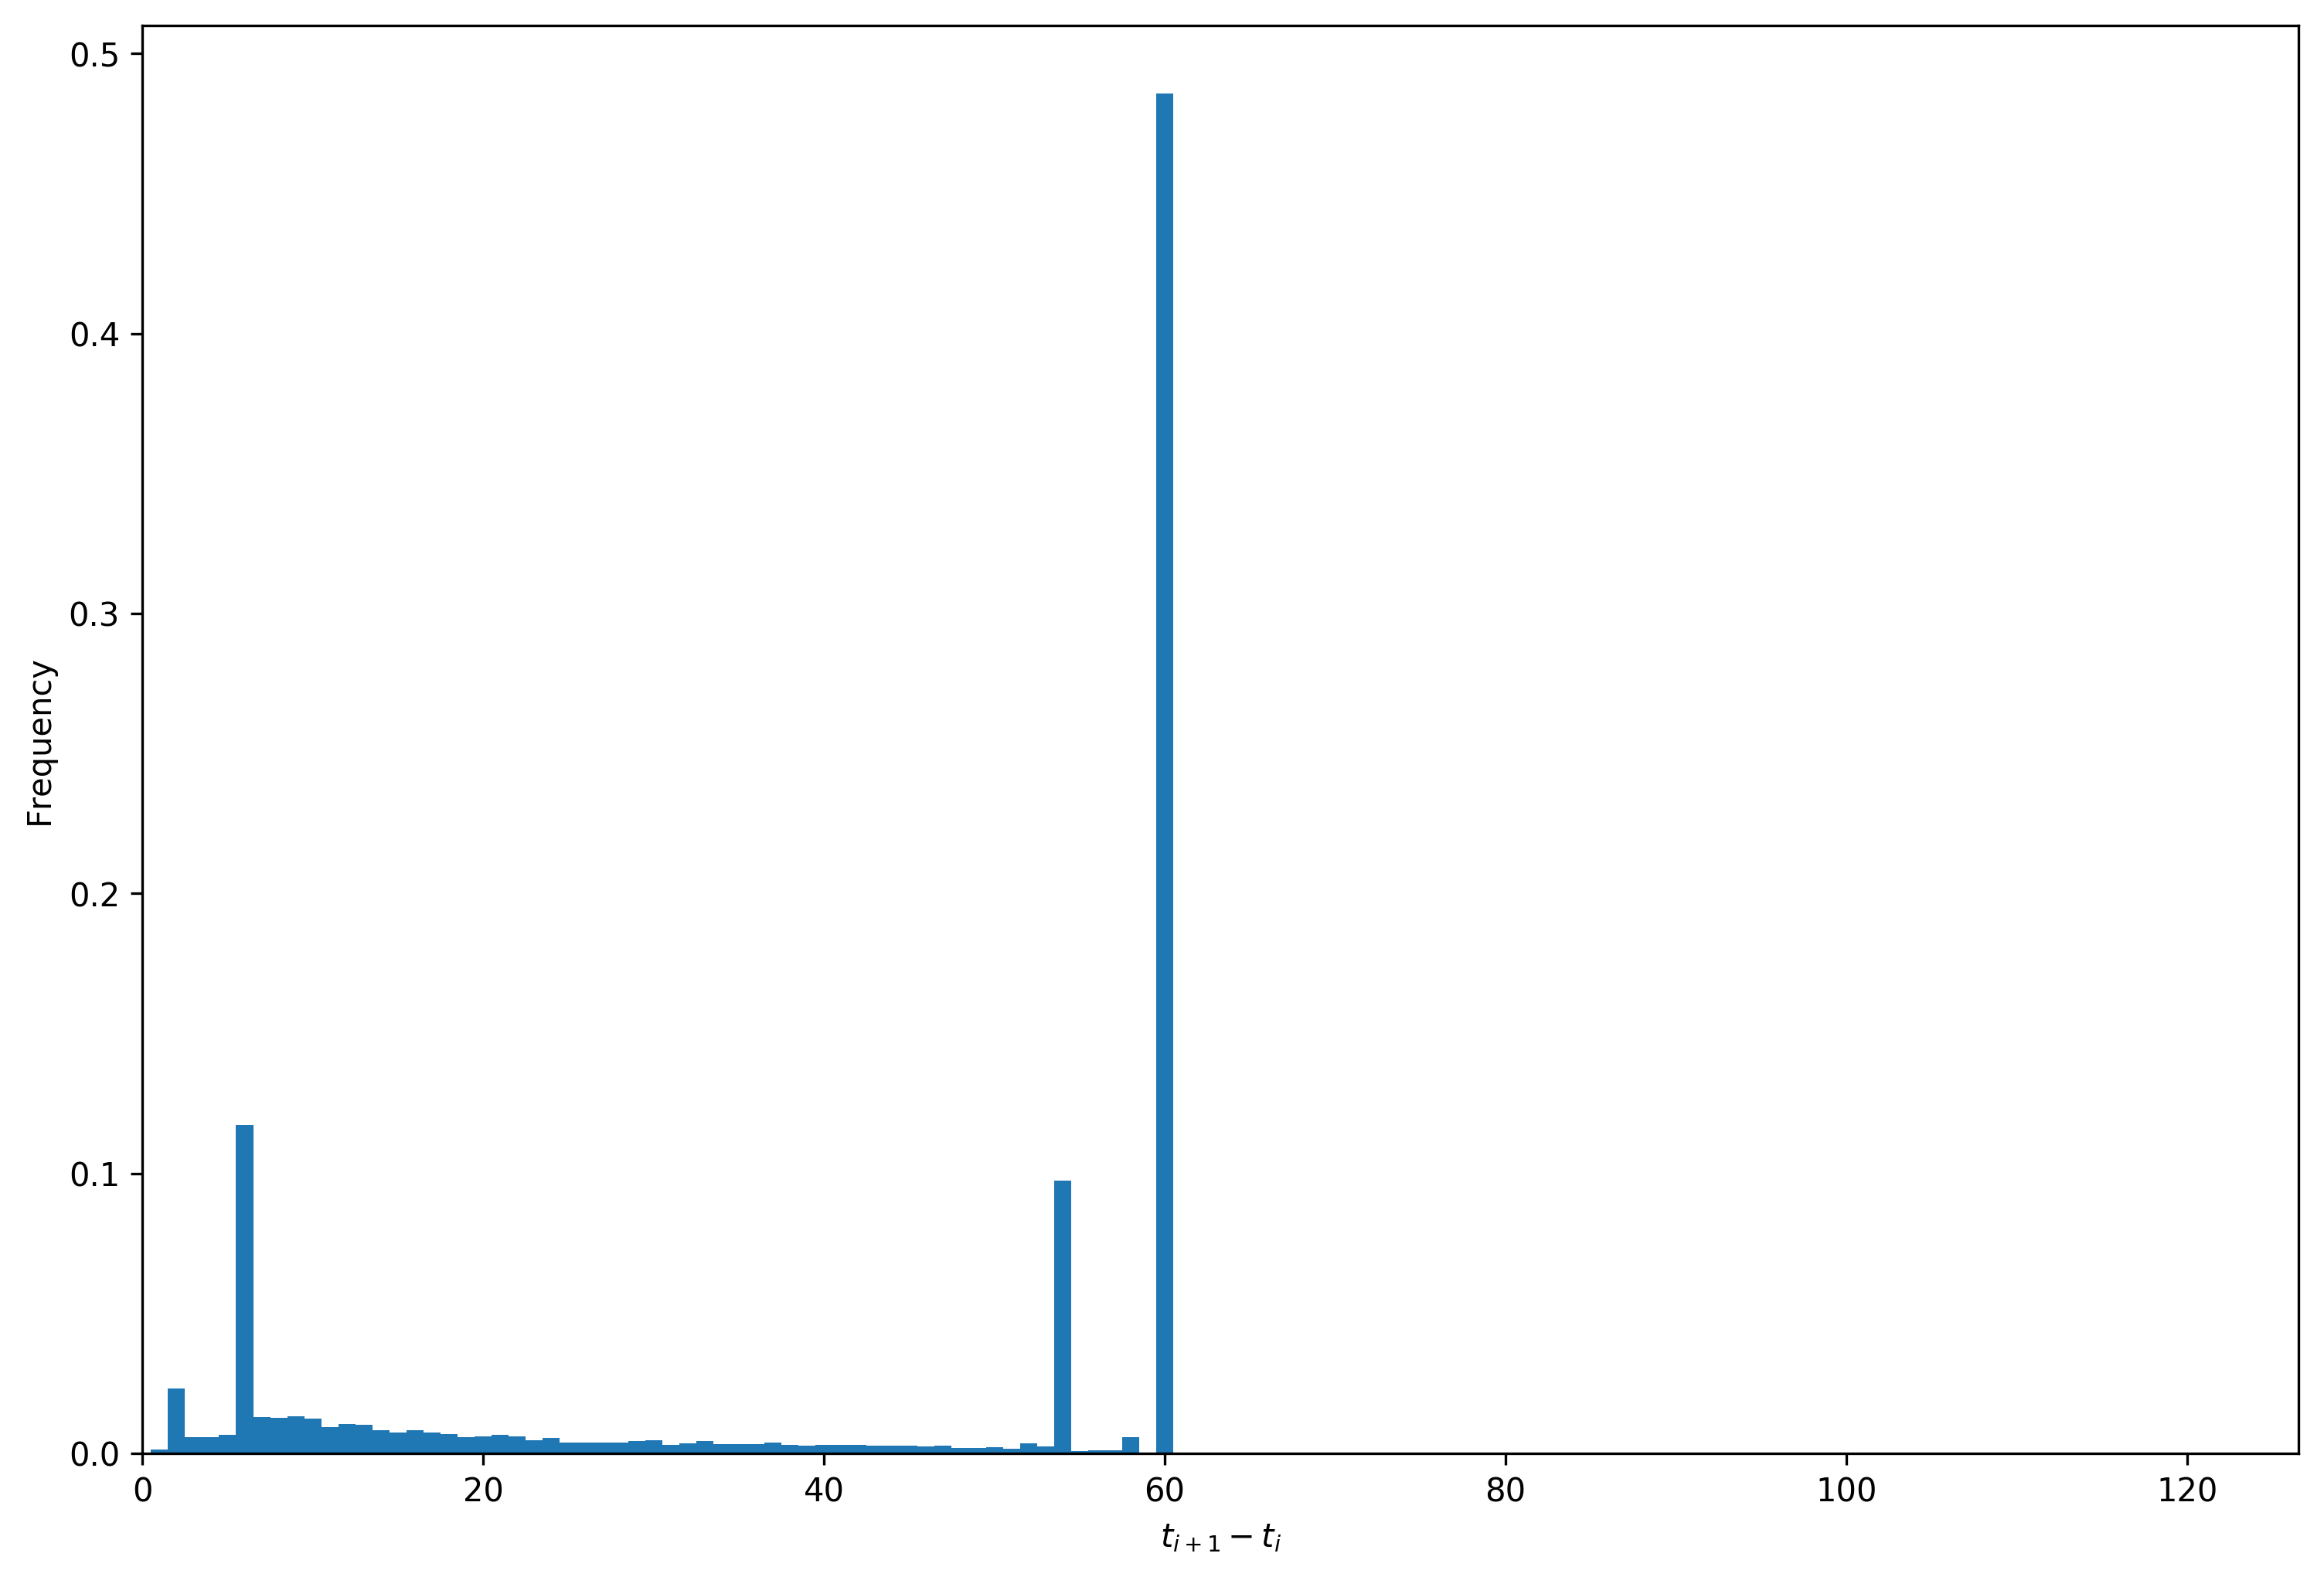
\includegraphics{../figures/histogram_time_diff.png}
\caption{\label{fig:histogram_time_diff}Histogram of time differences}
\end{figure}
    


        Because I already have imputations, it was easiest to apply this idea to the Waterloo Municipal Airport.
In that case I actually have access to hourly measurements, so I can compute the true \(\mean\del{\T_\miss}\).
The time series is provided as \(N=12,695\) measurements \(\T_{\miss,i}\), \(i=1,\dotsc,N\) made at times \(t_i\).
I refer to these as hourly measurements, but in reality the time series is irregular, with median difference of 54~minutes, mean difference 41.4 minutes, minimum difference 1~minute, and maximum difference 120 minutes (histogram in Figure~\ref{fig:histogram_time_diff}).
For this reason, we can't simply average the temperature measurements, we should weight each observation by the amount of time it occupies.
This gives weight

\begin{equation}
w_i = \begin{cases}
    \frac{1}{2}\del{t_{i+1}-t_i} & ,i=1 \\
    \frac{1}{2}\del{t_{i+1}-t_{i-1}} & ,i=2,\dotsc,N-1 \\
    \frac{1}{2}\del{t_{i}-t_{i-1}} & ,i = N
    \end{cases}
\end{equation}

to the \(i^\text{th}\) observation \(\T_{\miss,i}\).
Another way to write this, which turns out to be notationally more convenient, is to weight the temperature midpoints

\begin{equation}
    \midpoint\del{\T_{\miss}, i} \equiv \del{ \T_{\miss,i+1} + \T_{\miss,i} } \big/ 2 \,,i=1,\dotsc,N-1
\end{equation}

by the time differences

\begin{equation}
    \Delta_i = t_{i+1}-t_i\,.
\end{equation}

The weighted mean can therefore be written as:

\begin{equation}
    \mean\del{\T_\miss} 
        \approx 
        \mean\del{
            \cbr{
                \del{\T_{\miss,i},t_i}: \,i=1,\dotsc,N
            }
        }
        \equiv 
        \frac{1}{t_N - t_1} \sum_{i=1}^{N-1} \midpoint\del{\T_{\miss}, i} \Delta_i
\label{eq:weighted_mean}
\end{equation}

Applying this weighted mean formula to the temperatures measured at Waterloo Municipal Airport yields an annual mean of \(\mean\del{\T_\miss} = 9.497\,\degreeC\) in 2015.
    


        \textbf{Conventional estimate of mean temperature at Waterloo Airport}

\begin{figure}
\centering
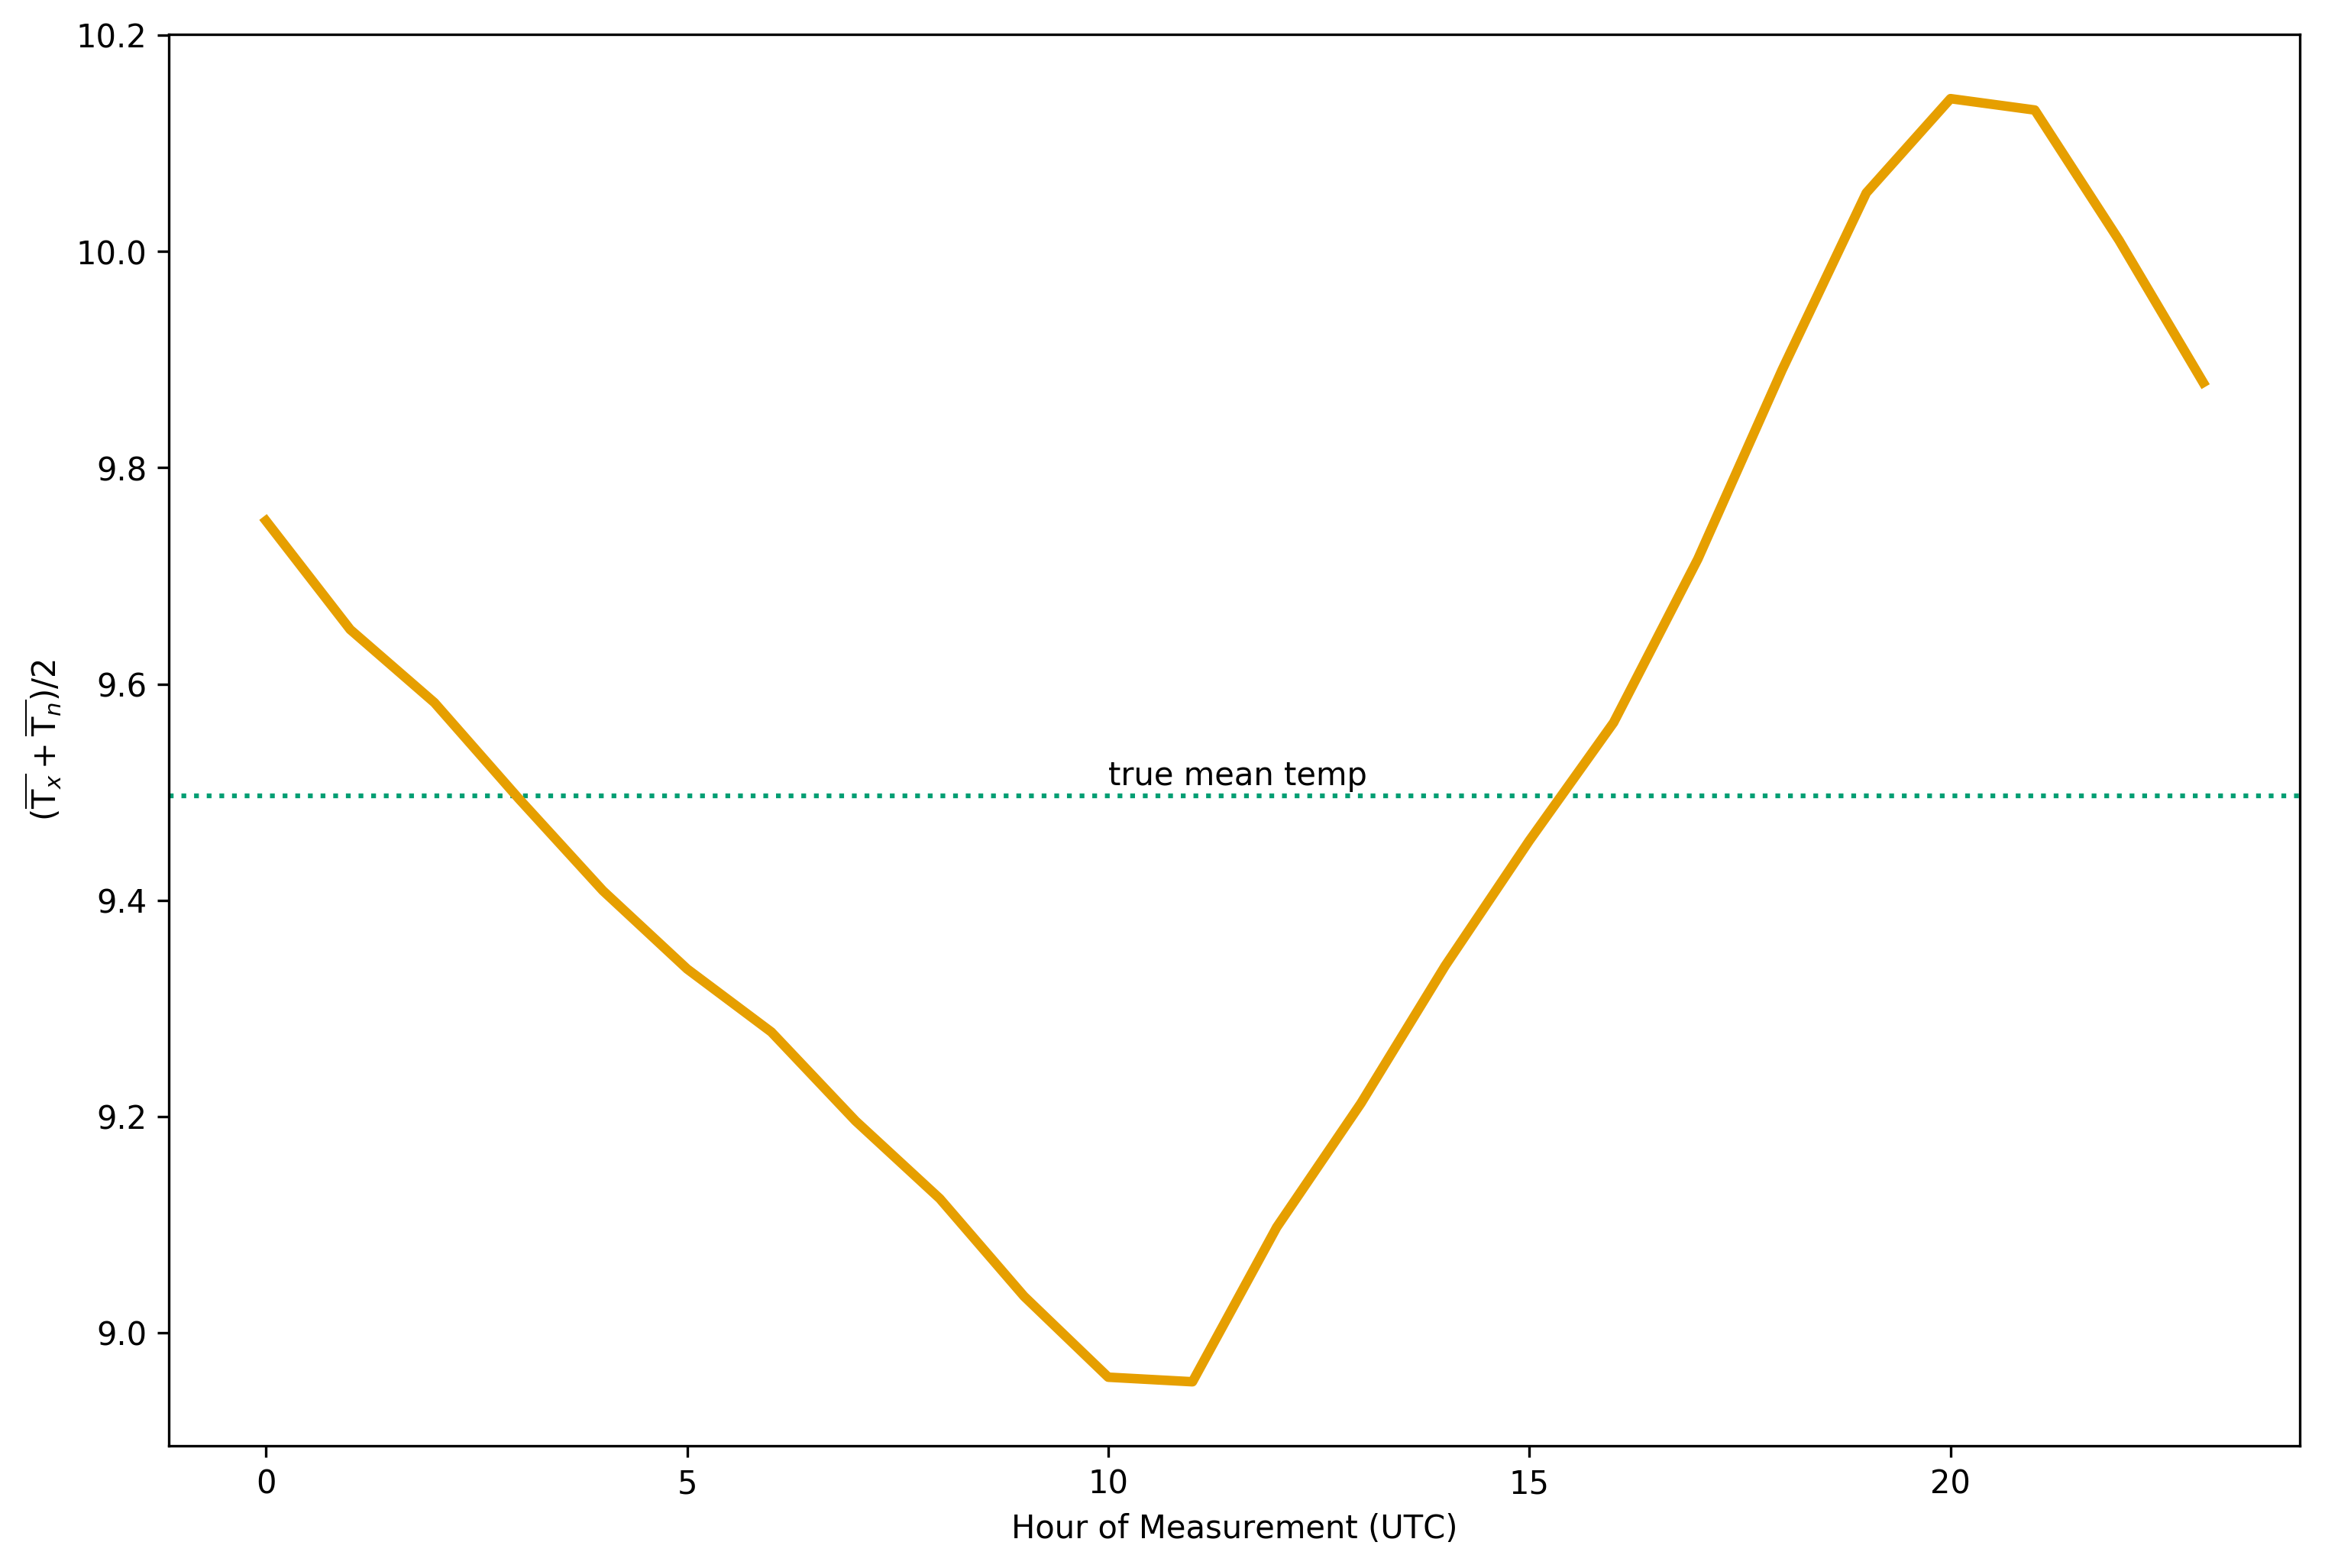
\includegraphics{../figures/waterloo_mean_temp_by_hour.png}
\caption{\label{fig:waterloo_mean_temp_by_hour}The 2015 mean temperature at Waterloo Municipal Airport conventionally estimated by averaging \(\Tn\) and \(\Tx\) depends on the hour of measurement.}
\end{figure}
    


        The conventional approach to estimating \(\mean\del{\T_\miss}\) is to average the daily \(\Tn\) and \(\Tx\) measurements.
At Waterloo Airport, since we have \(\T_\miss\), we can emulate this by first obtaining \(\Tn\del{\T_\miss, \hour}\), \(\Tx\del{\T_\miss, \hour}\) and then averaging the results together.
The result depends on \(\hour\), and so I show the results as a function of \(\hour\) in Figure~\ref{fig:waterloo_mean_temp_by_hour}.
Strikingly, the estimate varies by over \(1\,\degreeC\) depending on the hour of measurement.
If the \(\Tn\)/\(\Tx\) measurements are made at 17:00~UTC, the average temperature will be estimated as \(9.716\,\degreeC\).
    


        \textbf{Imputation-based estimate of mean temperature at Waterloo Airport}
    


        Now I go ahead and apply the \(\mean\) function to the imputations.
This isn't quite so straightforward because for computational reasons I obtained the temperature imputations for 2015 in nine-day windows, with three days overlap between adjacent windows.
What follows is some mildly painful notation to make it completely clear how I'm obtaining my imputation-based estimate.
We denote the time interval covered by the \(k^\text{th}\) window as \(\window_k\), so \(\cbr{i:\,t_i \in \window_k}\) is the indices of the observations that are within this window.
Each observation can fall in multiple windows.
For a given time \(t\) and a window \(k\), I can calculate the buffer \(\buffer(t; k) = \min\del{\max\del{\window_k} - t, t - \min\del{\window_k}}\) that separates the time \(t\) and the window's closest edge.
The best window for imputing an observation at time \(t\) is then found by \(\argmax_k \del{\buffer\del{t; k}}\).
And the set of indices of the midpoints (times halfway between two observations) for which window \(k\) is the best is then written as:

\begin{equation}
\best_k \equiv
\cbr{
    i: \argmax_{k'} \del{\buffer\del{\midpoint\del{t, i}; k'}} = k
}\,.
\end{equation}

Those midpoints occupy a duration of \(\timespan\del{\best_k} = t_{\max\del{\best_k}+1} - t_{\min\del{\best_k}}\).
For the \(l^\text{th}\) imputed time series \(\T_\miss^{(l)}\) (\(l=1,\dotsc,L\)) within each window \(k\), I obtain the weighted mean of imputed temperatures for the midpoints in the middle of the window:

\begin{equation}
    \overline{\T}_{k}^{(l)} = \mean\del{
            \cbr{
                \del{\T_{\miss,i}^{(l)},t_i} ;\,i \in \best_k
            }
        }
         \,,
\end{equation}

as defined in \eqref{eq:weighted_mean}.
The posterior mean and variance \(\mu_k\), \(\sigma^2_k\) are estimated by computing the sample mean and variance of \(\overline{\T}_{k}^{(l)}\) over the \(L\) imputations.
Then I combine the estimates for each window by taking a weighted mean of the \(\mu_k\)'s:

\begin{equation}
\begin{split}
    \E\del{\mean\del{\T_\miss} \mid \Tn, \Tx, \T_\obs, \hour} 
    &=
    \frac{1}{t_N - t_1} \sum_{k=1}^K \mu_k \timespan\del{\best_k} \\
    \var\del{\mean\del{\T_\miss} \mid \Tn, \Tx, \T_\obs, \hour} 
    &\approx \frac{1}{\del{t_N - t_1}^2} \sum_{k=1}^K \sigma^2_k \timespan\del{\best_k}^2 \\
\end{split}
\end{equation}

The expectation of the posterior of \(\mean\del{\T_\miss}\) is exact up to Monte Carlo error, but the variance estimate ignores correlations between windows.
Long story short, the resulting estimate is

\begin{equation}
\begin{split}
    \E\del{\mean\del{\T_\miss} \mid \Tn, \Tx, \T_\obs, \hour} 
    &=
    9.474\,\degreeC\\
    \var\del{\mean\del{\T_\miss} \mid \Tn, \Tx, \T_\obs, \hour} 
    &\approx \del{0.020\,\degreeC}^2\,, \\
\end{split}
\end{equation}

which is a good estimate of the true \(\mean\del{\T_\miss} = 9.497\,\degreeC\).
    



    % Add a bibliography block to the postdoc
    
    
\bibliographystyle{ametsoc2014}
\bibliography{temperature_imputations}

    
    \end{document}
